\begin{frame}
  \frametitle{Otras métricas}
  \framesubtitle{de entrainment prosódico}
  \begin{itemize}
    \item La mimetización es un fenómeno tanto lineal: se va acentuando a lo largo de la conversación
    \item Pero también es un fenómeno dinámico: va variando localmente a lo largo de la conversación.
  \end{itemize}

  Muchas métricas sólo toman la parte global, dividiendo la conversación en 2 o más partes y luego calculando la diferencia entre las medias de las diferentes variables acústicas en cada sección.

  Otros problema que tienen algunas métricas es que no son automáticas: requieren de anotaciones manuales sobre las conversaciones, por ejemplo patrones de entonación.
\end{frame}


\begin{frame}
  \frametitle{Problema del alineamiento de tiempo}

  \begin{figure}[t]
    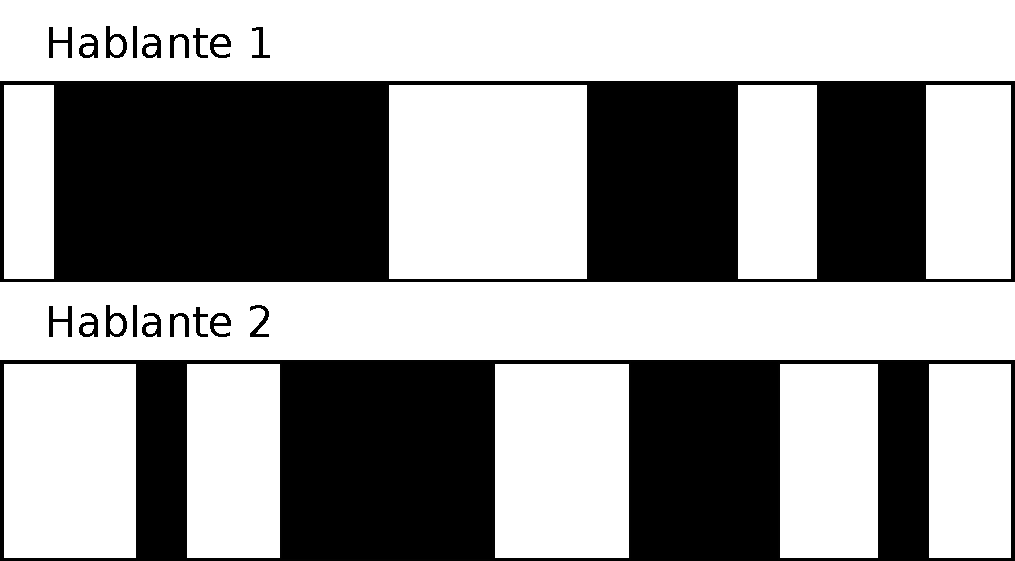
\includegraphics[scale=0.40]{images/conversation_turns.pdf}
  \end{figure}
  Uno de los problemas que tenemos a la hora de construir métricas de entrainment

  \begin{itemize}
    \item ¿Cómo comparamos los diferentes turnos de una conversación?
    \item Comparar uno a uno es un enfoque simplista y no representativo de la realidad
  \end{itemize}
\end{frame}

\begin{frame}
  \frametitle{Problema de la escala}

  Otro problema que podemos tener es de escalas: por ejemplo, si un hablante es de sexo femenino, su tono será más alto que el de un hombre.

\end{frame}



\begin{frame}
  \frametitle{Método TAMA}
  \begin{itemize}
    \item El método TAMA (Time aligned moving average) ataca estos problemas recién mencionados para la medición de entrainment acústico/prosódico
    \item ¿Cómo? Construye en primer lugar series de tiempo para cada uno de los hablantes, dada una variable acústico/prosódica.
    \item Luego aplica herramientas de análisis de series de tiempo para definir alguna medida de entrainment
  \end{itemize}
\end{frame}


\begin{frame}
  \frametitle{Series de Tiempo}
  \framesubtitle{¿Qué es una serie de tiempo?}

  \begin{figure}[t]
    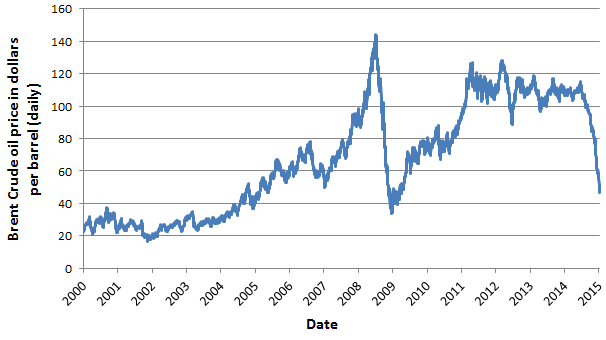
\includegraphics[scale=0.35]{images/oil_price.jpg}
  \end{figure}

  \begin{itemize}
     \item En términos coloquiales, una serie de tiempo es una colección de datos temporales.
     \item Muy frecuentes en Economía y Ciencias de la Atmósfera.
     \item ¡Mucho más manejables que una sucesión de turnos!
   \end{itemize}
\end{frame}



\begin{frame}
  \frametitle{Método TAMA}
  \framesubtitle{Cómo construyo la serie de tiempo (dada una variable a-p)}
  \begin{figure}[t]
    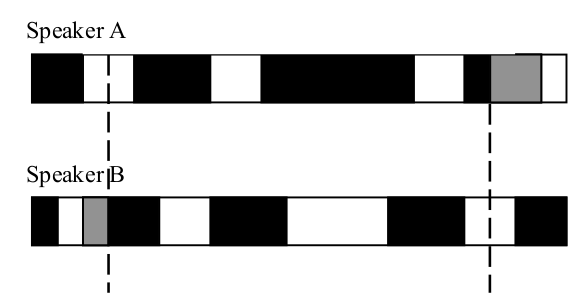
\includegraphics[scale=0.25]{images/tama.png}
  \end{figure}


  \begin{enumerate}
    \item Partimos la conversación en ventanas solapadas.
    \item Calculamos un promedio ponderado del valor de la variable acústico-prosódica en cada segmento de habla
  \end{enumerate}

  \begin{align*}
    \mu = \frac{\sum\limits_{i=1}^N f_i d_i}{\sum\limits_{i=1}^N d_i}
  \end{align*}
\end{frame}


\begin{frame}
  \frametitle{Método TAMA}
  \framesubtitle{¿Y el entrainment?}
  \begin{columns}
  \column{0.33\textwidth}
  \begin{figure}[t]
    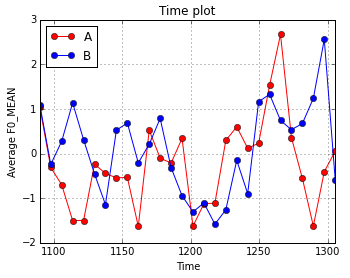
\includegraphics[scale=0.28]{images/time_plot.png}
  \end{figure}
  \begin{figure}[t]
    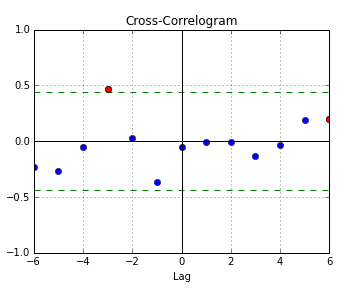
\includegraphics[scale=0.28]{images/cross_correlogram.png}
  \end{figure}
  \column{0.66\textwidth}
  \begin{enumerate}
    \item Ya tenemos la serie de tiempo
    \item ¿Cómo calculamos la mimetización?
    \item Función de correlación cruzada: mide la influencia de una serie sobre otra.
    \item Similar a la correlación, pero aplicando un desplazamiento en alguna de las dos series.
    \item Los valores significativos de esta son los que se consideran los valores de \emph{entrainment} (si es que los hay)
  \end{enumerate}

  \end{columns}
\end{frame}
